% ── Autentifikácia ────────────────────────────────────────────
\chapter{Autentifikácia}

        Autentifikácia je prvým krokom, ktorým prechádza každý používateľ systému.
Zabezpečuje, že k~citlivým projektovým dátam a~dokumentom môžu pristupovať len
oprávnené osoby. Systém sme implementovali pomocou knižnice Flask-Login~\cite{flask_login} s~dôrazom
na bezpečnosť prihlasovacieho procesu.

\section{Registrácia}

        Registráciu nových používateľov sme zámerene obmedzili pozývacím kódom.
Tento mechanizmus zabraňuje neautorizovaným osobám vytvoriť si konto a~zabezpečuje,
že do systému sa dostanú len skutočne pozvaní členovia tímu.

        Postup registrácie:

\begin{itemize}
  \item Používateľ otvorí registračný formulár a~zadá meno, e-mailovú adresu,
        heslo a~pozývací kód.
  \item Systém overí správnosť pozývacieho kódu (porovnaním s~hodnotou \texttt{REGISTRATION\_INVITE\_CODE}
        v~konfigurácii).
  \item Heslo je zahashované pomocou funkcie \texttt{generate\_password\_hash} z~Werkzeug~\cite{werkzeug_docs}
        pred uložením do databázy. Pôvodné heslo sa nikdy neukladá.
  \item Po úspešnej registrácii je používateľovi pridelená predvolená rola a~je
        presmerovaný na prihlasovanie (obr.~
ef{fig:registracia}).
\end{itemize}

\begin{figure}[H]
  \centering
  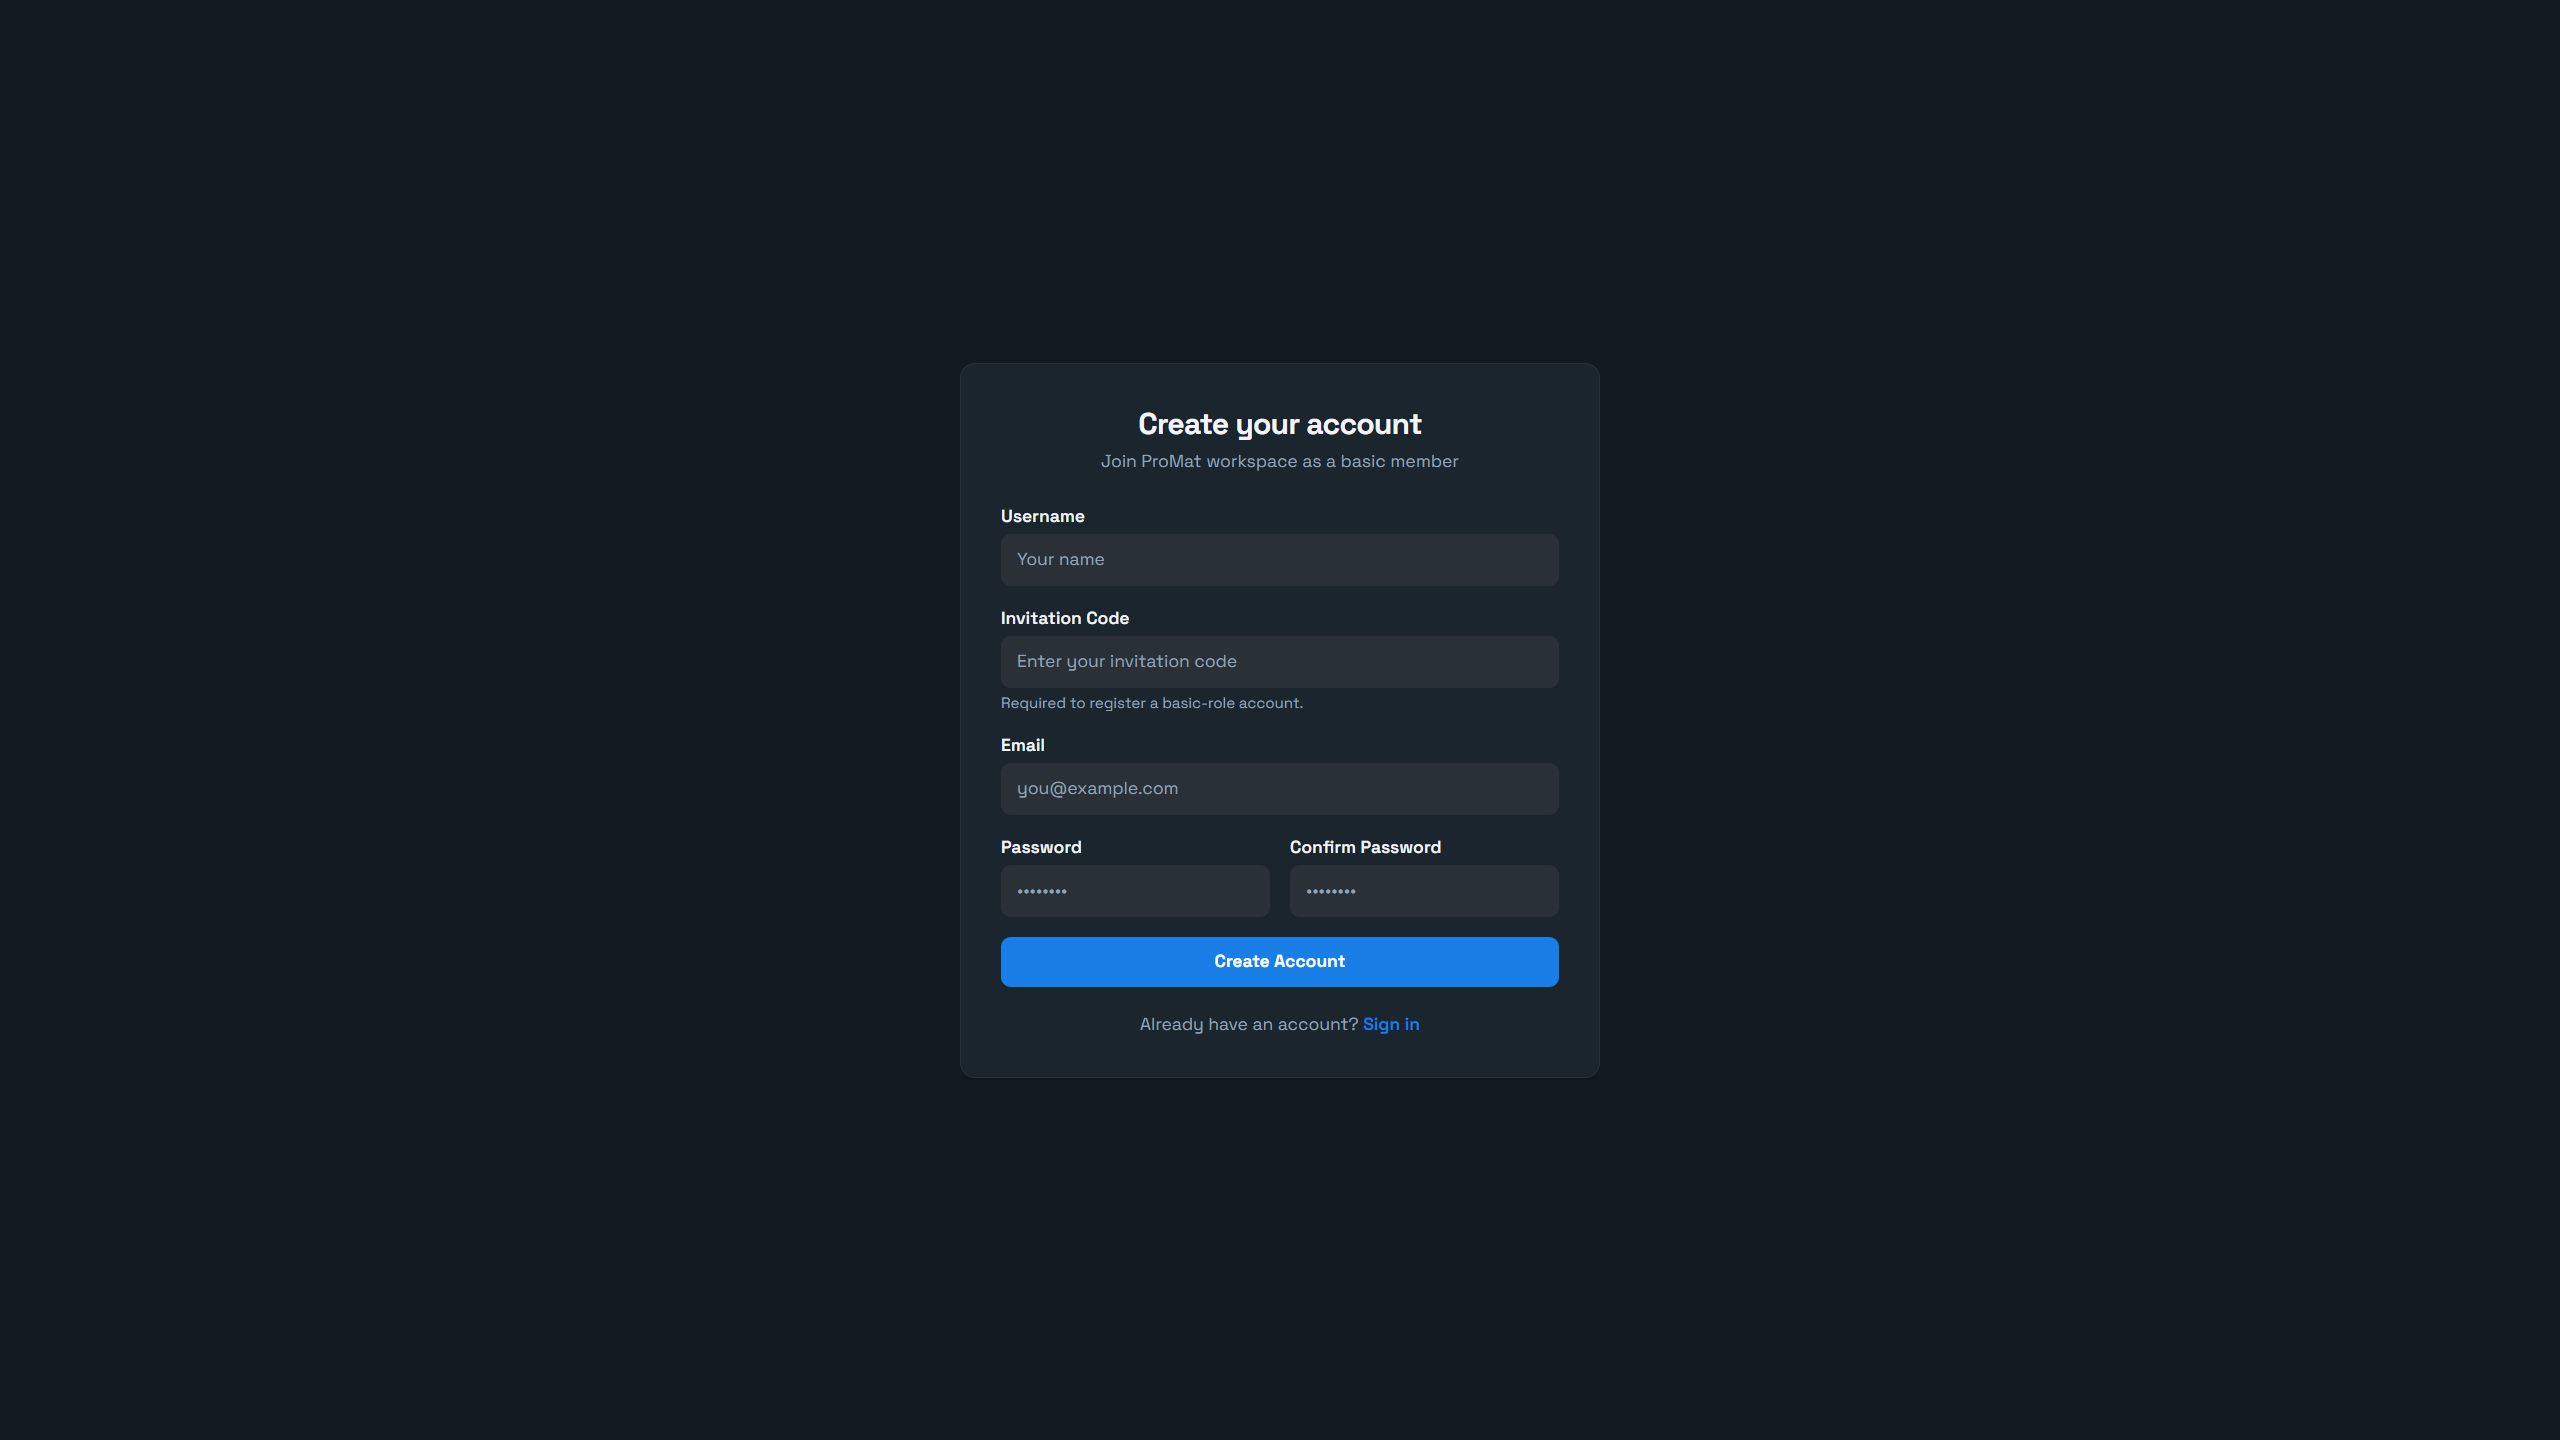
\includegraphics[width=0.75\textwidth]{images/registracia.png}
  \caption{Registračný formulár}
  \label{fig:registracia}
\end{figure}

\section{Prihlásenie}

        Prihlasovací proces overuje totožnosť používateľa porovnaním zadaných
prihlasovacích údajov s~uloženými hodnotami v~databáze.

        Postup prihlásenia:

\begin{itemize}
  \item Používateľ zadá e-mailovú adresu a~heslo do prihlasovacieho formulára.
  \item Flask-Login overí, či používateľ s~daným e-mailom existuje v~databáze.
  \item Werkzeug funkcia \texttt{check\_password\_hash} porovná zadané heslo
        s~uloženým hashom.
  \item Pri úspešnom prihlásení Flask-Login vytvorí reláciu a~uloží informáciu
        o~prihlásenom používateľovi do HTTPS session cookie.
  \item Pri nesprávnych údajoch systém zobrazí chybové hlásenie bez prezradenia,
        ktorý z~údajov je nesprávny (obr.~
ef{fig:prihlasenie}).
\end{itemize}

        Systém obsahuje aj vstavaného administrátora, ktorého prihlasovacie údaje
sme nakonfigurovali cez premenné prostredia (\texttt{BUILTIN\_ADMIN\_USERNAME},
\texttt{BUILTIN\_ADMIN\_EMAIL}, \texttt{BUILTIN\_ADMIN\_PASSWORD}). Tento
administrátor sa vytvorí automaticky pri prvom spustení aplikácie.

\begin{figure}[H]
  \centering
  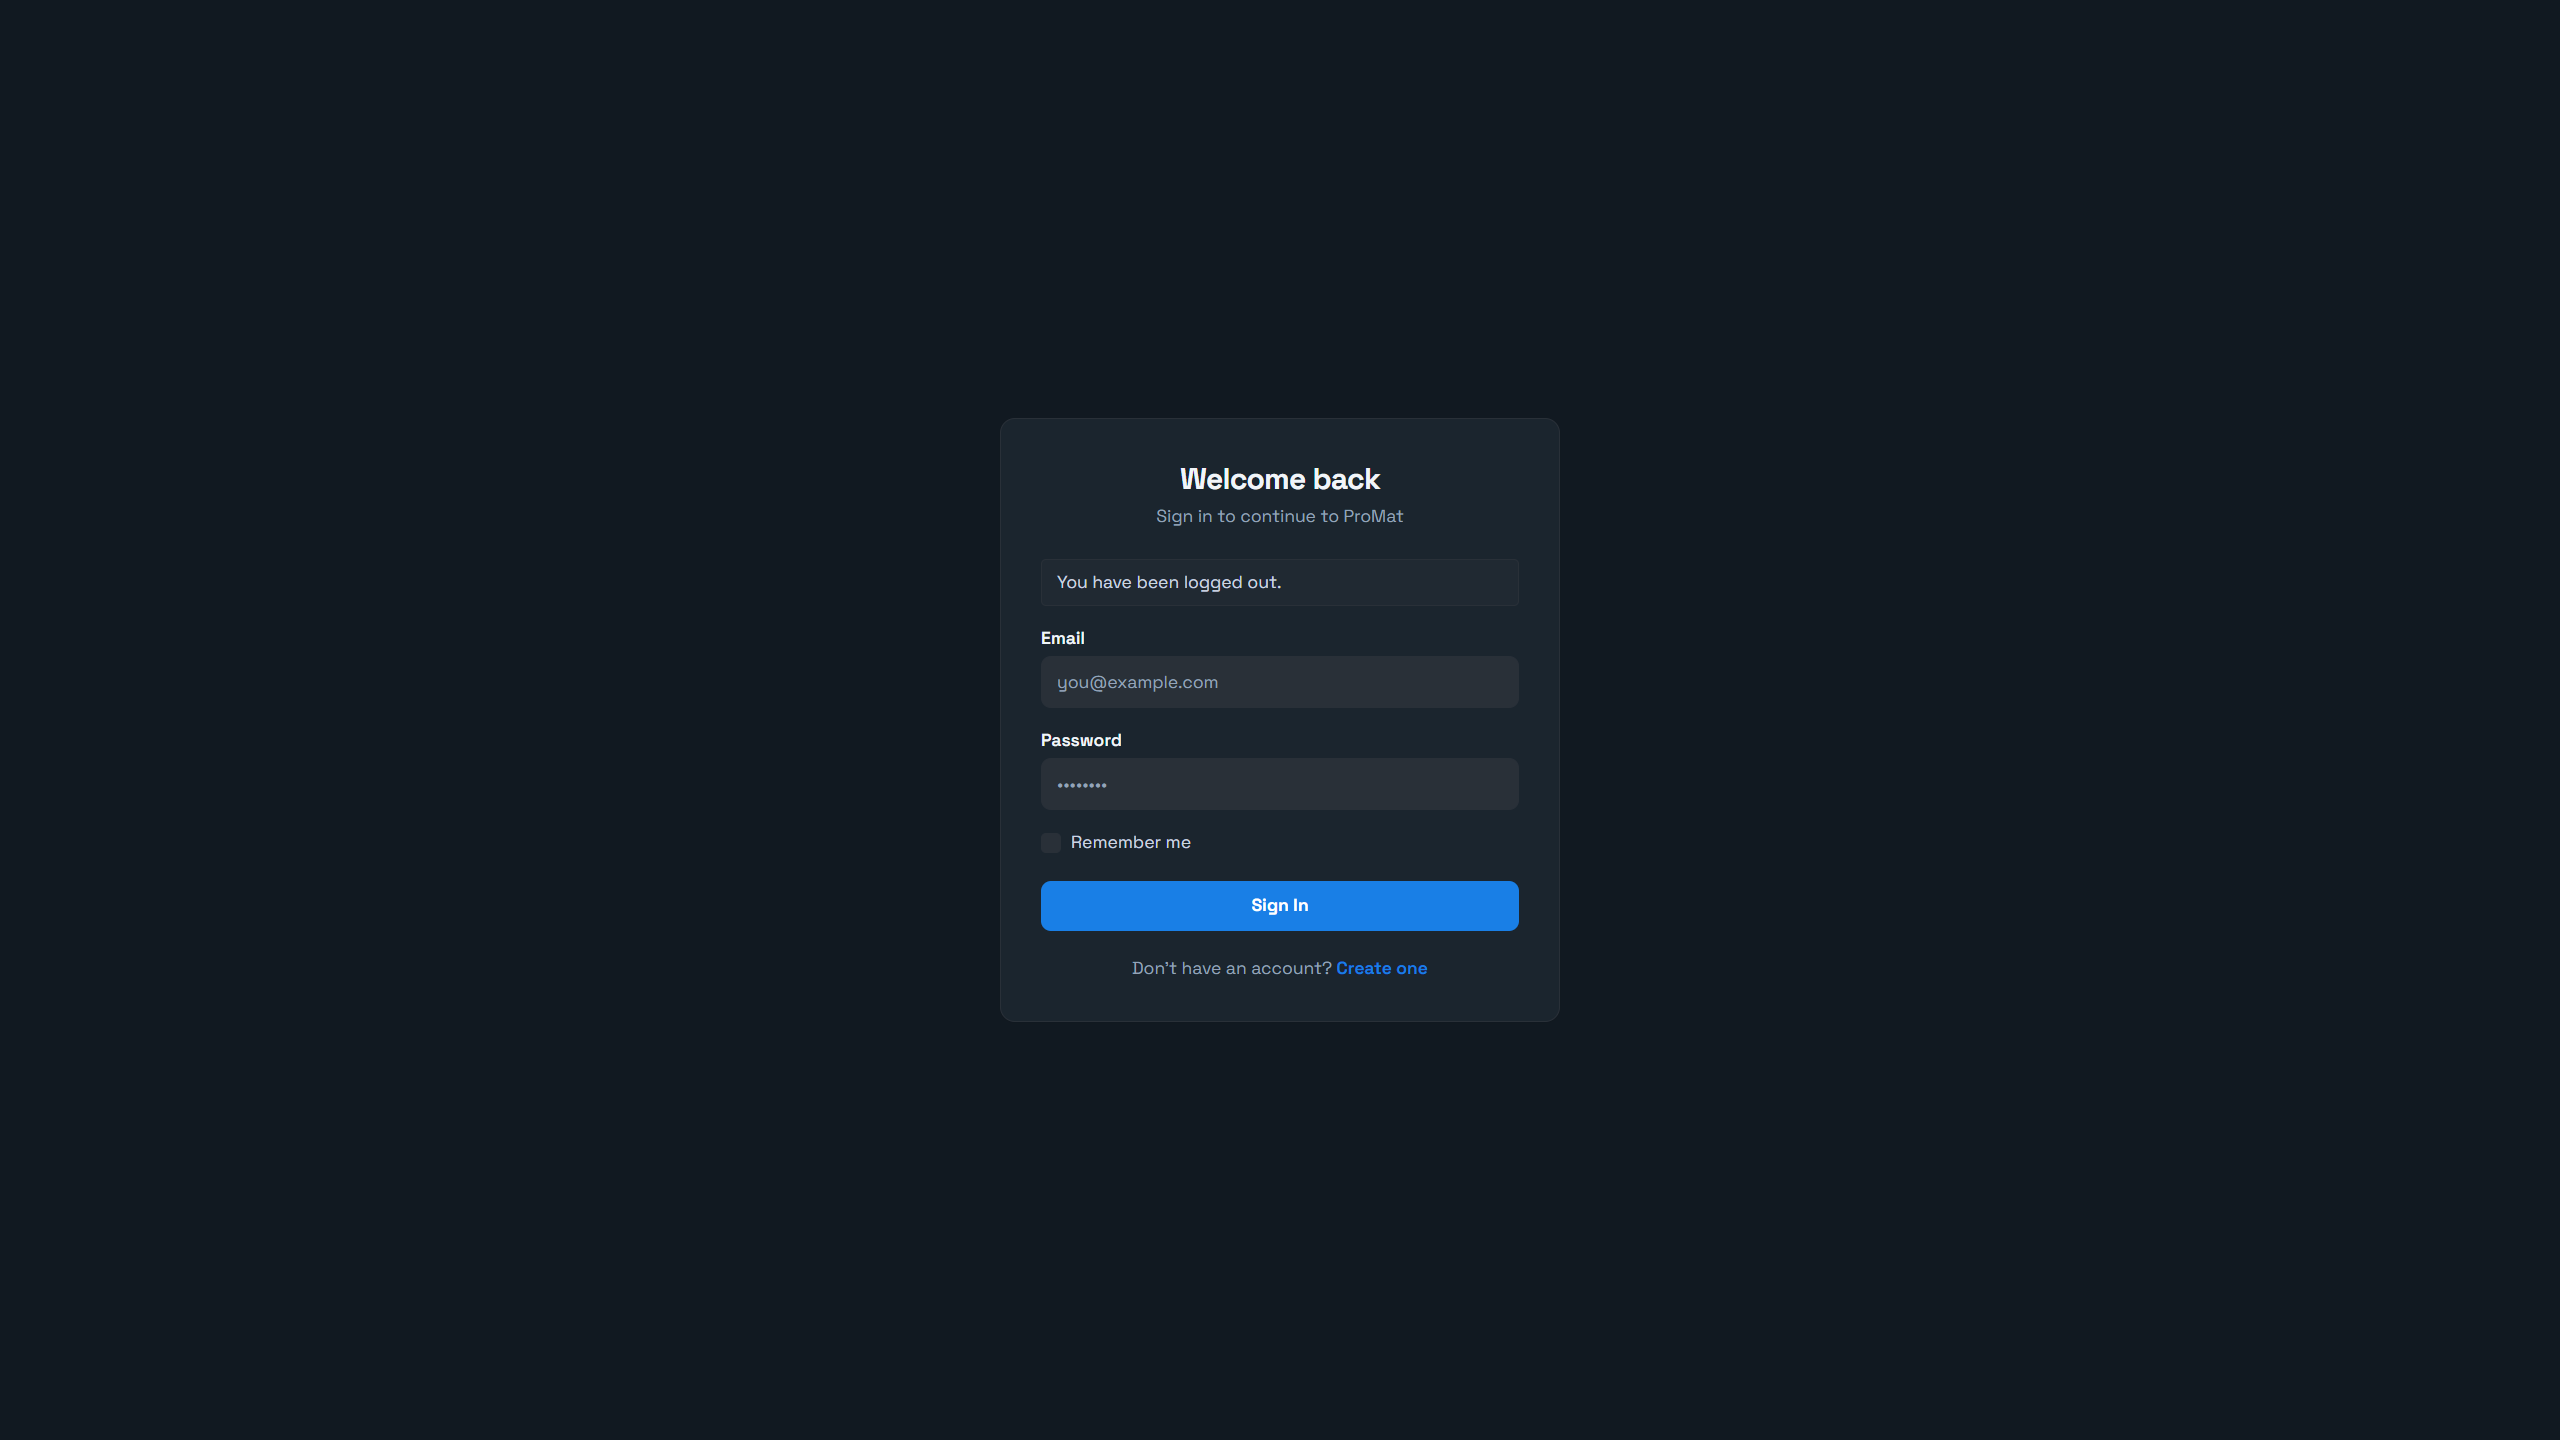
\includegraphics[width=0.75\textwidth]{images/prihlasenie.png}
  \caption{Prihlasovací formulár}
  \label{fig:prihlasenie}
\end{figure}

\section{Správa relácie}

        Po úspešnom prihlásení Flask-Login udržiava reláciu používateľa počas
celej práce s~aplikáciou.

        Všetky chránené stránky (routes označené dekorátorom \texttt{@login\_required})
automaticky presmerujú neprihlásených používateľov na prihlasovací formulár.
Po prihlásení sú používatelia presmerovaní späť na pôvodne požadovanú stránku.

        Odhlásenie prebieha manuálne cez odkaz v~navigácii. Flask-Login vymaže
reláciu a~presmeruje používateľa na prihlasovací formulár. Na ochranu formulárov
pred CSRF útokmi sme využili Flask-WTF~\cite{flask_wtf}, ktorý automaticky generuje a~overuje
CSRF token pri každom odoslaní formulára.
